\documentclass[
  captions=tableheading,
  bibliography=totoc, 
  titepage=firstiscover,
]{scrartcl}

\usepackage{blindtext} %neuer input

\usepackage{longtable} % Tabellen über mehrere Seiten

\usepackage[utf8]{inputenc} %neuer input

\usepackage{scrhack}

\usepackage[aux]{rerunfilecheck} %Warnung falls nochmal kompiliert werden muss

\usepackage{fontspec} %Fonteinstellungen

\recalctypearea{}

\usepackage[main=ngerman]{babel} %deutsche Spracheinstellung

\usepackage{ragged2e} %neuer input

\usepackage{amsmath, nccmath}

\usepackage{amssymb} %viele mathe Symbole

\usepackage{mathtools} %Erweiterungen für amsmath


\DeclarePairedDelimiter{\abs}{\lvert}{\rvert}
\DeclarePairedDelimiter{\norm}{\lVert}{\rVert}

\DeclarePairedDelimiter{\bra}{\langle}{\rvert}
\DeclarePairedDelimiter{\ket}{\lvert}{\rangle}

\DeclarePairedDelimiterX{\braket}[2]{\langle}{\rangle}{
#1 \delimsize| #2
}

\NewDocumentCommand \dif {m}
{
\mathinner{\symup{d} #1}
}


\usepackage[
  math-style=ISO,
  bold-style=ISO,
  sans-style=italic,
  nabla=upright,
  partial=upright,
  warnings-off={
    mathtools-colon,
    mathtools-overbracket,
  },
]{unicode-math}

\setmathfont{Latin Modern Math}
\setmathfont{XITS Math}[range={scr, bfscr}]
\setmathfont{XITS Math}[range={cal, bfcal}, StylisticSet=1]


\usepackage[
  locale=DE,
  separate-uncertainty=true,
  per-mode=reciprocal,
  output-decimal-marker={,},
]{siunitx}

\usepackage[autostyle]{csquotes} %richtige Anführungszeichen

\usepackage{xfrac}

\usepackage{float}

\floatplacement{figure}{htbp}

\floatplacement{table}{htbp}

\usepackage[ %floats innerhalb einer section halten
  section,   %floats innerhalb er section halten
  below,     %unterhalb der Section aber auf der selben Seite ist ok
]{placeins}

\usepackage[
  labelfont=bf,
  font=small,
  width=0.9\textwidth,
]{caption}

\usepackage{subcaption} %subfigure, subtable, subref

\usepackage{graphicx}

\usepackage{grffile}

\usepackage{booktabs}

\usepackage{microtype} %Verbesserungen am Schriftbild

\usepackage[
backend=biber,
]{biblatex}

\addbibresource{../lit.bib}

\usepackage[ %Hyperlinks im Dokument
  german,
  unicode,
  pdfusetitle,
  pdfcreator={},
  pdfproducer={},
]{hyperref}

\usepackage{bookmark}

\usepackage[shortcuts]{extdash}

%\usepackage{warpcol}

\allowdisplaybreaks

\begin{document}
    \title{Physik IV Übungsblatt 3}
    \author{  
    Tobias Rücker\\
    \texorpdfstring{\href{mailto:tobias.ruecker@tu-dortmund.de}{tobias.ruecker@tu-dortmund.de}
    \and}{,} 
    Paul Störbrock\\
    \texorpdfstring{\href{mailto:paul.stoerbrock@tu-dortmund.de}{paul.stoerbrock@tu-dortmund.de}}{}
    }
\maketitle
\center{\Large Abgabegruppe: \textbf{4H}}
\thispagestyle{empty}

\newpage
\tableofcontents
\thispagestyle{empty}
\newpage

\setcounter{page}{1}

\section{Aufagabe 1}

\begin{figure}[H]
    \centering
    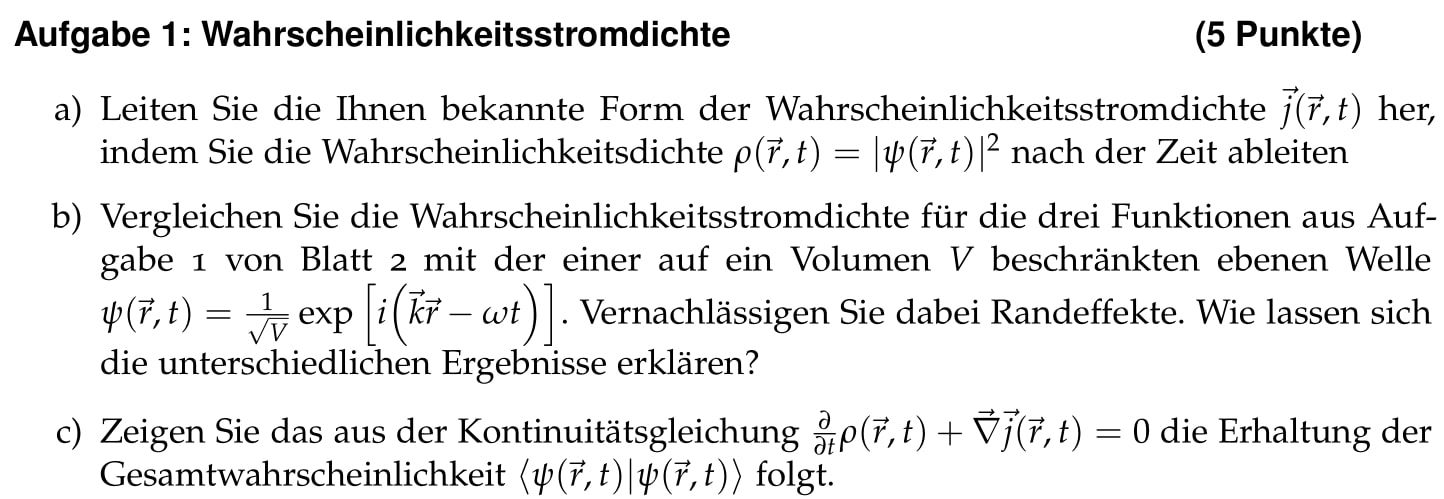
\includegraphics[width=0.75\textwidth]{./images/Aufgabe1.jpg}
    \label{fig:1}
\end{figure}

\subsection{a)}

    \begin{align*}
        \rho(\vec{r},t) &= \abs{\psi(\vec{r},t)}^2\\
        \frac{\partial\rho(\vec{r},t)}{\partial t} &= \frac{\partial}{\partial t} \abs{\psi(\vec{r},t)}^2\\
        &= \frac{\partial}{\partial t} (\psi^* \cdot \psi)\\
        &= \left( \psi^* \frac{\partial}{\partial t} \psi + \psi \frac{\partial}{\partial t} \psi^* \right)\\
        \frac{\partial \psi}{\partial t} &= \frac{1}{i\hbar} \left( -\frac{\hbar^2}{2m} \nabla^2 \psi + V\psi \right)\\
        &= - \frac{i\hbar}{2m}\nabla^2 \psi - \frac{i}{\hbar} V \psi\\
        \frac{\partial \psi^*}{\partial t} &= -\frac{i\hbar}{2m} \nabla^2 \psi^* + \frac{i}{\hbar} V \psi^*\\
        &= \psi^* \left( \frac{i\hbar}{2m} \nabla^2 \psi - \frac{i}{\hbar} V \psi \right) + \psi \left( -\frac{i\hbar}{2m} \nabla^2 \psi^* + \frac{i}{\hbar} V \psi^* \right)\\
        &= \frac{i\hbar}{2m} \psi^* \nabla^2 \psi \underbrace{\,-\,\frac{i}{\hbar} V \abs{\psi}^2}_{\text{Wegk\"urzen}} - \frac{i\hbar}{2m} \psi \nabla^2 \psi^* \underbrace{\,+\,\frac{i}{\hbar} V \abs{\psi}^2}_{\text{Wegk\"urzen}}\\
        &= - \nabla \underbrace{\left( \frac{\hbar}{2m} \left( \psi^* \nabla \psi - \psi \nabla \psi^* \right) \right)}_{\vec{j}} \tag{*}\\
        &= - \nabla \vec{j}\\
        \frac{\partial}{\partial t}\rho &= -\nabla\vec{j} 
    \end{align*}

\newpage
\subsection{b)}

    \flushleft{Die\;}\justifying folgenden Zustände werden dem Übungsblatt 2 entnommen:

    \noindent\makebox[\linewidth]{\rule{\textwidth}{1pt}}
    \begin{align*}
        \text{I} \qquad \psi_1 &= N_1 \exp \left(-\frac{x^2}{2x_0^2} \right),\\
        \text{II} \qquad \psi_2 &= N_2 \frac{x}{x_0} \exp \left( -\frac{x^2}{2x_0^2} \right),\\
        \text{III} \qquad \psi_3 &= N_3 \left( 2\frac{x^2}{x_0^2}-1 \right) \exp \left( -\frac{x^2}{2x_0^2} \right)
    \end{align*}
    \noindent\makebox[\linewidth]{\rule{\textwidth}{1pt}}

    \begin{align*}
        \vec{j_1} &\stackrel{(*)}{=} \left( \frac{\hbar}{2m} \left( \psi_1^* \nabla \psi_1 - \psi_1 \nabla \psi_1^* \right) \right)\\
        &\text{\noindent\makebox[\linewidth]{\rule{\linewidth}{0.4pt}}}\\
        &\nabla \psi_1 = N_1 \exp \left(-\frac{x^2}{2x_0^2} \right)\\
        &\text{\noindent\makebox[\linewidth]{\rule{\linewidth}{0.4pt}}}\\
        &= \frac{\hbar}{2mi} \left( N_1^2 exp \left( -\frac{x^2}{x_0^2} \right) \frac{-x}{x_0^2} - N_1^2 exp\left( -\frac{x^2}{x_0^2} \right) \frac{-x}{x_0^2} \right)\\
        &= 0\\
        \\
        \vec{j_2} &\stackrel{(*)}{=} \left( \frac{\hbar}{2m} \left( \psi_2^* \nabla \psi_2 - \psi_2 \nabla \psi_2^* \right) \right)\\
        &\text{\noindent\makebox[\linewidth]{\rule{\linewidth}{0.4pt}}}\\
        &\nabla \psi_2 = N_2 \left( \frac{1}{x_0^2} - \frac{x^2}{x_0^3} \right) \exp \left( - \frac{x^2}{2x_0^2} \right)\\
        &\text{\noindent\makebox[\linewidth]{\rule{\linewidth}{0.4pt}}}\\
        &= \frac{\hbar}{2mi} \left( N_2^2 \exp \left( -\frac{x^2}{x_0^2} \right) \left( \frac{1}{x_0} - \frac{x^2}{x_0^3} \right) - N_2^2 \exp \left( -\frac{x^2}{x_0^2} \right) \left( \frac{1}{x_0} - \frac{x^2}{x_0^3} \right)  \right)\\
        &= 0\\
        \\
        \vec{j_3} &\stackrel{(*)}{=} \left( \frac{\hbar}{2m} \left( \psi_3^* \nabla \psi_3 - \psi_3 \nabla \psi_3^* \right) \right)\\
        &\text{\noindent\makebox[\linewidth]{\rule{\linewidth}{0.4pt}}}\\
        \nabla \psi_3 &= N_3 \nabla \left( \left( \frac{2x^2}{x_0^2} -1 \right) \exp \left( -\frac{x^2}{2x_0^2} \right) \right)\\
        &= N_3 \left( \frac{4x}{x_0^2} + \left( \frac{2x^2}{x_0^2} - 1 \right) \left( -\frac{x}{x_0^2} \right) \right) \exp \left( -\frac{x^2}{2x_0^2} \right)\\
        &= N_3 \left( \frac{5x}{x_0^2} - \frac{2x^3}{x_0^4} \right) \exp \left( -\frac{x^2}{2x_0^2} \right)\\
        &\text{\noindent\makebox[\linewidth]{\rule{\linewidth}{0.4pt}}}\\
        &= \frac{\hbar}{2mi} \left( N_3^2 \exp \left( -\frac{x^2}{x_0^2} \right) \left( \frac{5x}{x_0^2} - \frac{2x^3}{x_0^4} \right) - N_3^2 \exp \left( -\frac{x^2}{x_0^2} \right) \left( \frac{5x}{x_0^2} - \frac{2x^3}{x_0^4} \right) \right)\\
        &= 0\\
        \\
        \Aboxed{\psi(\vec{r}, t) &= \frac{1}{\sqrt{V}} \exp \left[ i \left( \vec{k} \vec{r} - \omega t \right) \right]}\\
        \vec{j} &\stackrel{(*)}{=} \left( \frac{\hbar}{2mi} \left( \psi^* \nabla \psi - \psi \nabla \psi^* \right) \right)\\
        &\text{\noindent\makebox[\linewidth]{\rule{\linewidth}{0.4pt}}}\\
        \nabla \psi(\vec{r}, t) &= \frac{1}{\sqrt{V}} i\vec{k} \exp \left[ i \left( \vec{k} \vec{r} - wt \right) \right]\\
        \nabla \psi^*(\vec{r}, t) &= \frac{1}{\sqrt{V}} (-i)\vec{k} \exp \left[ -i \left( \vec{k} \vec{r} - wt \right) \right]\\
        &\text{\noindent\makebox[\linewidth]{\rule{\linewidth}{0.4pt}}}\\
        &= \frac{\hbar}{2mi} \left( \frac{1}{V} i\vec{k} - \frac{1}{V} (-i)\vec{k} \right)\\
        \vec{j} &= \frac{\hbar}{Vm}\, \vec{k}
    \end{align*}

\newpage
\subsection{c)}

    \begin{align*}
        \frac{\partial}{\partial t} \rho &= -\nabla \cdot \vec{j}\\
        \frac{\partial}{\partial t} \abs{\psi}^2 &= - \nabla \cdot \vec{j}\\
        \frac{\partial}{\partial t} \int_{-\infty}^{\infty}  \abs{\psi}^2 \,\mathrm{d}x &= -\int_{\symbb{R}} \nabla \cdot \vec{j} \,\mathrm{d}V\\
        &= \vec{j}\, \vert_{\symbb{R}}\\
        &\stackrel{(*)}{=} \left( \frac{\hbar}{2mi} \left( \psi^* \nabla \psi - \psi \nabla \psi^*   \right) \right) \big| _{\symbb{R}}\\
        \frac{\partial}{\partial t} \int_{-\infty}^{\infty} \abs{\psi}^2 &= 0\\
        \frac{\partial}{\partial t} \langle \psi(\vec{r}, t) \vert \psi(\vec{r}, t) \rangle &= 0
    \end{align*}

\section{Aufgabe 2}

\begin{figure}[H]
    \centering
    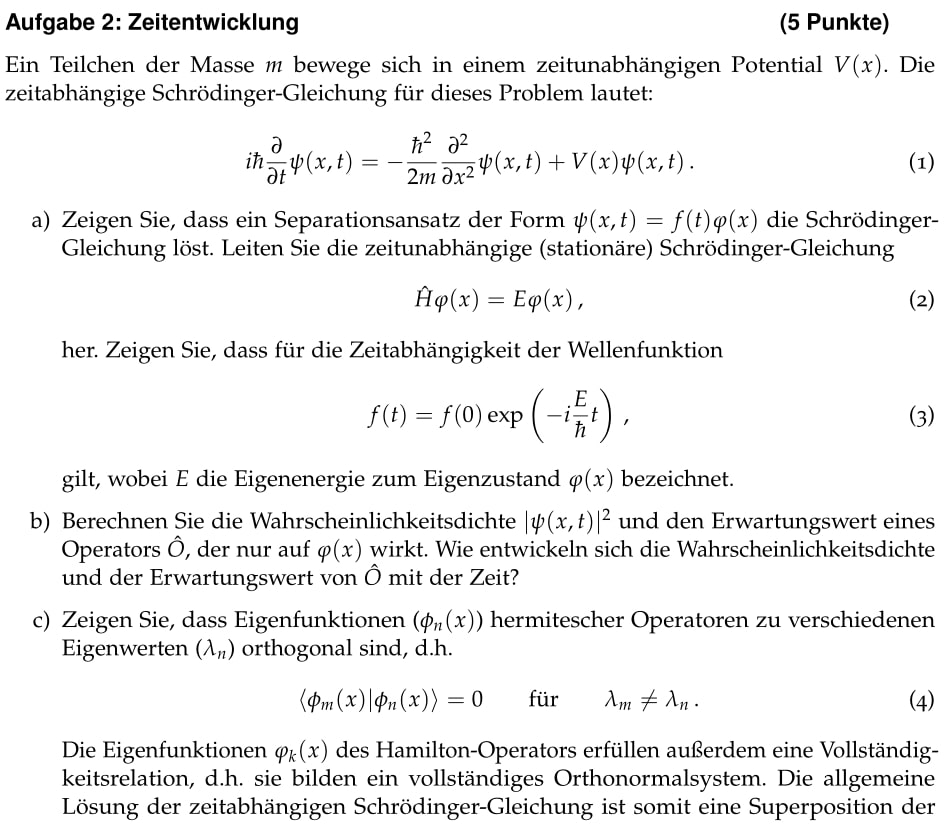
\includegraphics[width=0.75\textwidth]{./images/Aufgabe2abc.jpg}
    \label{fig:2}
\end{figure}

\begin{figure}[H]
    \centering
    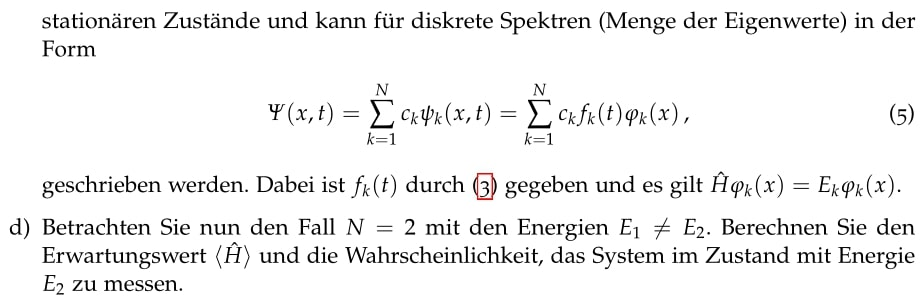
\includegraphics[width=0.75\textwidth]{./images/Aufgabe2d.jpg}
    \label{fig:3}
\end{figure}

\subsection{a)}

    \begin{align*}
        i\hbar \frac{\partial}{\partial t} \psi(x, t) &= -\frac{\hbar^2}{2m} \frac{\partial^2}{\partial x^2} \psi(x, t) + V(x) \psi(x, t)\\
        \\
        \psi(x, t) &= f(t)\varphi(x)\\
        \\
        i\hbar \varphi(x) \frac{\partial}{\partial t} f(t) &= -\frac{\hbar^2}{2m} f(t) \frac{\partial^2}{\partial x^2} \varphi(x) + V(x) \varphi(x) f(t) \qquad \vert :\varphi(x)f(x)\\
        \underbrace{i\hbar \frac{1}{f(t)} \frac{\partial}{\partial t}f(t)}_{\text{Nur t-abh\"angig}} &= \underbrace{-\frac{\hbar^2}{2m} \frac{1}{\varphi(x)} \frac{\partial^2}{\partial x^2} \varphi(x) + V(x)}_{\text{Nur x-abh\"angig}}\\
        \Rightarrow E &= -\frac{\hbar^2}{2m} \frac{1}{\varphi(x)} \frac{\partial^2}{\partial x^2} \varphi(x) + V(x)\\
        E \varphi(x) &= \frac{(-i\hbar)^2}{2m} \frac{\partial^2}{\partial x^2} \varphi(x) + V(x) \varphi(x)\\
        &= \frac{\hat{p}^2}{2m} \varphi(x) + V(x) \varphi(x)\\
        \hat{H} &= \frac{\hat{p}^2}{2m} + V\\
        \Rightarrow E \varphi(x) &= \hat{H} \varphi(x)\\
        \\
        i\hbar \frac{1}{f(x)} \frac{\partial}{\partial t} f(t) &= E\\
        \frac{\partial}{\partial t} f(t) &= -\frac{E}{\hbar} i f(t)\\
        f(t) &= f(0) \exp \left( -\frac{E}{\hbar} it \right)
    \end{align*}

\newpage
\subsection{b)}

    \begin{align*}
        \psi(x, t) &= f(0) \exp \left( -\frac{E}{\hbar} it \right) \varphi(x)\\
        \abs{\psi(x, t)}^2 &= \psi^* \psi = \abs{f(0)}^2 \exp \left( -\frac{E}{\hbar} it \right) \exp \left( \frac{E}{\hbar} it \right) \abs{\varphi(x)}^2\\
        &= \abs{f(0)}^2 \abs{\varphi(x)}^2\\
        \\
        \langle \psi(x, t) \vert \hat{O} \psi(x, t) \rangle &= \langle f(0) \varphi(x) \exp \left( -\frac{E}{\hbar} it \right) \vert \hat{O} f(0) \varphi(x) \exp \left( -\frac{E}{\hbar} it \right) \rangle\\
        &= \langle f(0) \varphi(x) \vert \hat{O} f(0) \varphi(x) \rangle\\
        &= \abs{f(0)}^2 \; \langle \varphi(x) \vert \hat{O} \phi(x) \rangle
        \intertext{F\"ür alle Zust\"ände, die nur auf $\varphi(x)$ wirken, folgt, dass der  Erwartungswert und für alle Zeiten gleich ist.
        Auch die Wahrscheinlichkeitsdichte ist ebenso zeitunanhängig.
        }
    \end{align*}


\subsection{c)}



\subsection{d)}

    \begin{align*}
        \langle \hat{H} \rangle &= \langle \psi_k(x, t) \vert \hat{H} \vert \psi_k(x, t) \rangle\\
        &= \langle c_1 \psi_1(x, t) + c_2 \psi_2(x, t) \vert \hat{H} \vert c_1 \psi_1(x, t) + c_2 \psi_2(x, t) \rangle\\
        \\
        &= \langle c_1 \psi_1(x, t) \vert \hat{H} \vert c_1 \psi_1(x, t) \rangle 
        + \langle c_1 \psi_1(x, t) \vert \hat{H} \vert c_2 \psi_2(x, t) \rangle
        + \langle c_2 \psi_2(x, t) \vert \hat{H} \vert c_1 \psi_1(x, t) \rangle\\
        &+ \langle c_2 \psi_2(x, t) \vert \hat{H} \vert c_2 \psi_2(x, t) \rangle\\
        \\
        &= \langle c_1 f_1(t) \varphi_1(x) \vert \hat{H} \vert c_1 f_1(t) \varphi_1(x) \rangle 
        + \langle c_1 f_1(t) \varphi_1(x) \vert \hat{H} \vert c_2 f_2(t) \varphi_2(x) \rangle
        + \langle c_2 f_2(t) \varphi_2(x) \vert \hat{H} \vert c_1 f_1(t) \varphi_1(x) \rangle\\
        &+ \langle c_2 f_2(t) \varphi_2(x) \vert \hat{H} \vert c_2 f_2(t) \varphi_2(x) \rangle\\
        \\
        &= \langle c_1 f_1(t) \varphi_1(x) \vert c_1 f_1(t) \hat{H} \varphi_1(x) \rangle
        + \langle c_1 f_1(t) \varphi_1(x) \vert c_2 f_2(t) \hat{H} \varphi_2(x) \rangle
        + \langle c_2 f_2(t) \varphi_2(x) \vert c_1 f_1(t) \hat{H} \varphi_1(x) \rangle\\
        &+ \langle c_2 f_2(t) \varphi_2(x) \vert c_2 f_2(t) \hat{H} \varphi_2(x) \rangle\\
        \\
        &= \langle c_1 f_1 \varphi_1 \vert c_1 f_1 E_1 \varphi_1 \rangle
        + \langle c_1 f_1 \varphi_1 \vert c_2 f_2 E_2 \varphi_2 \rangle
        + \langle c_2 f_2 \varphi_2 \vert c_1 f_1 E_1 \varphi_1 \rangle\\
        &+ \langle c_2 f_2 \varphi_2 \vert c_2 f_2 E_2 \varphi_2 \rangle\\
        \\
        &= \abs{c_1}^2 E_1 + \abs{c_2}^2 E_2\\
        \intertext{
            Die Wahrscheinlichkeit, dass $E_2$ gemessen wird, ist gleich dem Vorfaktor von E_2, also $\abs{c_2}^2 $:
        }
        \Rightarrow \abs{c_2}^2 &= 1 - \abs{c_1}
    \end{align*}

\section{Aufgabe 3}

\begin{figure}[H]
    \centering
    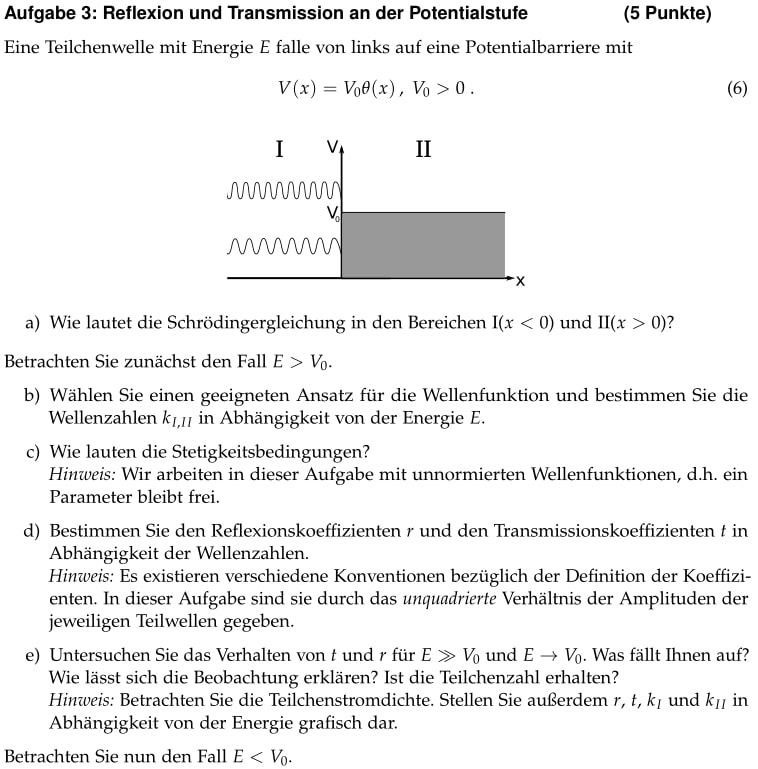
\includegraphics[width=0.75\textwidth]{./images/Aufgabe3a_e.jpg}
    \label{fig:4}
\end{figure}

\begin{figure}[H]
    \centering
    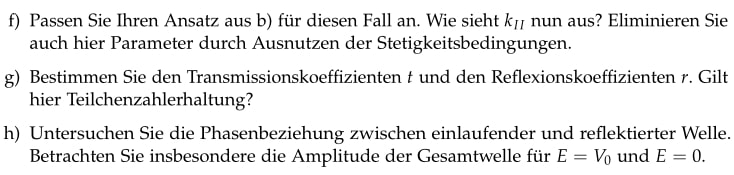
\includegraphics[width=0.75\textwidth]{./images/Aufgabe3f_h.jpg}
    \label{fig:5}
\end{figure}

\subsection{a)}

    \begin{align*}
        i\hbar \frac{\partial \psi}{\partial t} &= -\frac{\hbar}{2m} \frac{\partial \psi^2}{\partial x^2} + V \psi\\
        \intertext{Fallunterscheidung:
        }
        \intertext{Fall 1: $I(x<0) \Rightarrow V=0$
        }
        i\hbar \frac{\partial \psi}{\partial t} &= -\frac{\hbar}{2m} \frac{\partial \psi^2}{\partial x^2}
        \\
        \intertext{Fall 2: $I(x>0) \Rightarrow V=V_0\theta(x)$
        }
        i\hbar \frac{\partial \psi}{\partial t} &= -\frac{\hbar}{2m} \frac{\partial \psi^2}{\partial x^2} + V_0\theta(x) \psi
    \end{align*}

\subsection{b)}

    \begin{align*}
        \psi(x, t) =& f(t) g(x)\\
        i\hbar \theta \frac{\partial f}{\partial t} &= -\frac{\hbar^2}{2m} f \frac{\partial^2 g}{\partial x^2} + V g f \qquad \vert :\theta g\\
        \underbrace{i\hbar \frac{1}{f} \frac{\partial f}{\partial t}}_{E} &= -\frac{\hbar^2}{2m} \frac{1}{g} \frac{\partial^2 g}{\partial x^2} + V\\
        E &= -\frac{\hbar^2}{2m} \frac{1}{g} \frac{\partial^2 g}{\partial x^2} + V\\
        \Leftrightarrow \frac{\partial^2 g}{\partial x^2} &= -\frac{2m}{\hbar^2} (Eg + Vg)\\
        \\
        \intertext{Für $x \leq 0 \Rightarrow V=0:$
        }
        g_1 &= A \, exp(ik_1x) + B \, exp(-ik_1x)\\
        k_1 &= \sqrt{\frac{-2mE}{\hbar^2}} = \frac{\sqrt{-2mE}}{\hbar}\\
        \intertext{Für $x \geq 0:$
        }
        \frac{\partial^2 g_2}{\partial x^2} &= -\frac{2m}{\hbar^2}(E + V_0 \theta)g\\
        k_2 &= \frac{\sqrt{-2m(E+V_2 \theta)}}{\hbar}\\
        g_2 &= C \, exp(ik_2x) + D \, exp(-ik_2x)
    \end{align*}

\subsection{c)}

    \begin{align*}
        E &= i\hbar \frac{1}{f} \frac{\partial f}{\partial t} - \frac{V_0}{f}\\
        \Leftrightarrow \frac{1}{i\hbar} Ef &= \frac{\partial f}{\partial t}\\
        f &= c \; exp \left( -\frac{E}{\hbar}t \right)\\
        \\
        k \leq 0\\
        q_1 &= A \; exp(ik_1x) + B \; exp(-ik_1x)\\
        q_2 &= C \; exp(ik_2x) + D \; exp(-ik_2x)\\
        \intertext{Stetigkeit bei $x=0$
        }
        A + B &= C + D\\
        \frac{\mathrm{d}\psi}{\mathrm{d}x} \; \text{stetig bei $x=0$}\\
        &\text{Stetig}=\begin{cases}
            \frac{\mathrm{d} g_1}{\mathrm{d}x} = ik_1 (A\;exp(ik_1x) + B\;exp(-ik_1x)) \qquad \frac{\mathrm{d} g_1}{\mathrm{d}x} \vert_{-} = ik_1(A-B)\\
            \\
            \frac{\mathrm{d} g_2}{\mathrm{d}x} = ik_2 (C\;exp(ik_2x) + D\;exp(-ik_2x)) \qquad \frac{\mathrm{d} g_2}{\mathrm{d}x} \vert_{+} = ik_2(C-D)
        \end{cases}\\
        \Delta \left( \frac{\mathrm{d} g}{\mathrm{d}x} \right) &= i(k_1(A-B) -k_2(C-D)) =0\\
        A+B &= C+D \; \text{$D=0$ (Wellen laufen von links ein)}\\
        C &= A+B\\
        B &= C-A\\
        \\
        i(k_1(A-B) - k_2(+A+B)) &=0\\
        k_1(A-B) - k_2(+A+B) &=0\\
        -B(k_2+k_1) &= +(k_1+k_2)A\\
        \Leftrightarrow B &= -\frac{k_2-k_1}{k_2+k_1}A\\
        k_1(A-C+A)-k_2C &= 0\\
        \Leftrightarrow C &= \frac{2k_1}{k_2+k_1}A
    \end{align*}

\subsection{d)}

    \begin{align*}
        r  &= \frac{A}{B} = -\frac{k_2-k_1}{k_2+k_1}\\
        &= -\frac{\sqrt{-2m(E+V_0\theta)} - \sqrt{-2mE}}{\sqrt{-2m(E+V_0\theta)} + \sqrt{-2mE}}\\
        &= -\frac{\sqrt{E+V_0\theta} - \sqrt{E}}{\sqrt{E+V_0\theta} + \sqrt{E}}\\
        \\
        t &= \frac{C}{A} = \frac{2k_1}{k_1 + k_2}\\
        &= \frac{2\sqrt{-2mE}}{\sqrt{-2mE} + \sqrt{-2m(E+V_0\theta)}}\\
        &= \frac{2\sqrt{E}}{\sqrt{E} + \sqrt{-2m(E+V_0\theta)}}\\
        \\
        k_1 &= \frac{\sqrt{-2mE}}{\hbar}\\
        k_2 &= \frac{\sqrt{-2m(E+V_0\theta)}}{\hbar}
    \end{align*}

\subsection{e)}

    \begin{align*}
        \intertext{Fall $E \gg V_0  (V_0\;$ ist gegen\"uber E vernachl\"assigbar)
        }
        r &= 0\\
        t &= 1\\
        E \rightarrow V_0\\
        r &= \frac{\sqrt{1+\theta}-1}{\sqrt{1+\theta}+1}\\
        t &= \frac{2}{1+\sqrt{1+\theta}}
    \end{align*}

\subsection{f)}

    \begin{align*}
        V_0 > E \qquad x \leq 0\\
        g_1 &= A\;exp(k_1x) + B\;exp(-k_1x)\\
        \lim_{x \to -\infty} g_1 &= 0 \qquad \Rightarrow B=0\\
        g_1 &= A\;exp(k_1x)\\
        \\
        x \geq 0\\
        g_2 &= C\;exp(k_2x) + D\;exp(-k_2x)\\
        \lim_{x \to \infty} g_2 &= 0 \qquad \Rightarrow C=0\\
        g_2 &= D\;exp(-k_2x)
        \intertext{Stetigkeit:
        }
        A=D
        &\begin{cases}
            g_1(0)_L = A\cdot e^0\\
            \\
            g_2(0)_R = D\cdot e^0
        \end{cases}\\
        g(x)
        &\begin{cases}
            A\;exp(k_1x) \qquad x\leq 0\\
            \\
            A\;exp(-k_2x) \qquad x\geq 0
        \end{cases}\\
        \\
        -\frac{\hbar}{2m} \frac{\mathrm{d}^2 g}{\mathrm{d} x^2} - Vg &= Eg \qquad \lvert \int_{-\epsilon}^{\epsilon} \mathrm{d}x\\
        -\frac{\hbar}{2m} \int_{-\epsilon}^{\epsilon} \frac{\mathrm{d}^2 g}{\mathrm{d} x^2} \,\mathrm{d}x - \int_{-\epsilon}^{\epsilon} Vg \,\mathrm{d}x &= \underbrace{\int_{-\epsilon}^{\epsilon} Eg \,\mathrm{d}x}_{=0}\\
        \Delta \left( \frac{\mathrm{d} g}{\mathrm{d} x} \right) &= \lim_{\epsilon \to 0} \left( \frac{\mathrm{d} g}{\mathrm{d} x} \vert_{+\epsilon} - \frac{\mathrm{d} g}{\mathrm{d} x} \vert_{-\epsilon} \right)\\
        &= \frac{2m}{\hbar} \lim_{\epsilon \to 0} \int_{-\epsilon}^{\epsilon} V_0 \theta g(x) \mathrm{d}x\\
        \stackrel{Symmetrisch}{\Rightarrow} &= \frac{2m}{\hbar} V_0 \lim_{\epsilon \to 0} \int_{0}^{\epsilon} g(x) \mathrm{d}x\\
        &= \frac{2m}{\hbar} V_0 \lim_{\epsilon \to 0} \int_{0}^{\epsilon} A\;exp(-k_2x) \mathrm{d}x\\
        &= \frac{2m}{\hbar} V_0 \frac{1}{k_2} \lim_{\epsilon \to 0} A\;exp(-k_2x) \vert_0^{\epsilon}\\
        &= \frac{2m}{\hbar k_2} V_0 \lim_{\epsilon \to 0} \left( A\;exp(-k_2\epsilon) - A \right)\\
        &= 0
    \end{align*}

\subsection{g)}



\subsection{h)}





\end{document}